\documentclass[12pt, twoside]{article}
\usepackage[letterpaper, margin=1in, headsep=0.5in]{geometry}
\usepackage[english]{babel}
\usepackage[utf8]{inputenc}
\usepackage{amsmath}
\usepackage{amsfonts}
\usepackage{amssymb}
\usepackage{tikz}
%\usetikzlibrary{quotes, angles}

\usepackage{graphicx}
\usepackage{enumitem}
\usepackage{multicol}

\usepackage{fancyhdr}
\pagestyle{fancy}
\fancyhf{}
\renewcommand{\headrulewidth}{0pt} % disable the underline of the header

\fancyhead[LE]{\thepage}
\fancyhead[RO]{\thepage \\ Name: \hspace{4cm} \,\\}
\fancyhead[LO]{BECA / Dr. Huson / Geometry\\* Unit 7: Similarity\\* 9 January 2020}

\begin{document}
\subsubsection*{7.6b Classwork Mastery: Tangent function (collect 8 stars for each topic)\\[0.5cm]
Mastery topic: Interpreting tangent graphically}
  \begin{enumerate}
  \item Graph and label $\triangle ABC$ with $A(0,0)$, $B(5,5)$, and $C(5,0)$. Calculate each length:
    \begin{enumerate}[itemsep=1.25cm]
      \begin{multicols}{2}
      %\begin{enumerate}
        \item $AC=$ \hfill (1 star)
        \item $BC=$ \hfill (1 star)
        \item $AB=\sqrt{AC^2+BC^2}$ \hfill (2 stars) \vspace{2cm}
      %\end{enumerate}
    \begin{center}
      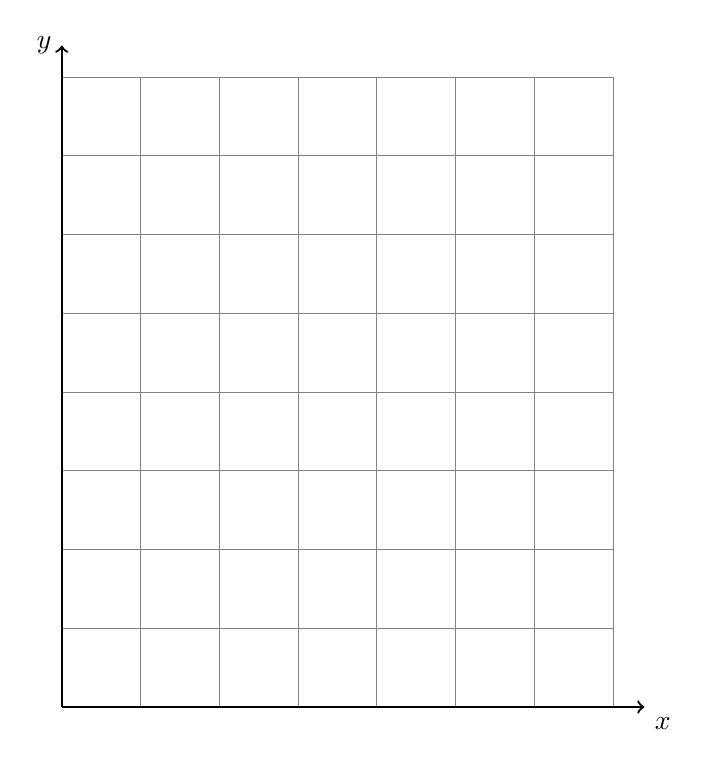
\begin{tikzpicture}%[scale=.635]
        \draw [help lines] (0,0) grid (7,8);
        \draw [thick, ->] (0,0) -- (7.4,0) node [below right] {$x$};
        \draw [thick, ->] (0,0)--(0,8.4) node [left] {$y$};
      \end{tikzpicture}
    \end{center}
    \end{multicols}\vspace{2cm}
      \item Use a protractor to measure $\angle BAC$ in degrees.  \hfill (1 star)
      \item The tangent of an angle is the ratio of the side lengths \emph{opposite} over \emph{adjacent} to the angle. Write down the value as a fraction.  \hfill (1 star)\\[0.5cm]
        $\tan \angle BAC=$
      \item Find $m\angle BAC$ with a calculator's inverse tangent function,\\ $\displaystyle m \angle BAC = \tan^{-1}(\frac{opp}{adj})$  \hfill (2 stars)
    \end{enumerate}

\newpage
\subsubsection*{Mastery topic: Algebraic solution \hfill (2 stars each)}
\item Solve each equation for $x$, rounding to the nearest hundredth.
  \begin{enumerate}
  \begin{multicols}{2}
  \item $\displaystyle \tan 63^\circ = \frac{x}{14}$ \vspace{5cm}
  \item $\displaystyle \tan 77^\circ = \frac{10}{x}$
  \item $\displaystyle \sin 46^\circ  = \frac{x}{3.5}$ \vspace{5cm}
  \item $\displaystyle \cos 35^\circ = \frac{x}{21}$ 
  \end{multicols}
\end{enumerate}
  \vspace{6cm}
\item Solve for $x$, rounding to the nearest whole degree.
  \begin{enumerate}
  \begin{multicols}{2}
  \item $\displaystyle x = \tan^{-1} (\frac{12}{5})$ \vspace{4cm}
  \item $\displaystyle \tan x^\circ = \frac{3.2}{4.8}$ \vspace{4cm}
  \end{multicols}
\end{enumerate}

\newpage
\subsubsection*{Mastery topic: Calculator use}
  \item Express the result to the nearest thousandth. \hfill (1 star each) \vspace{.5cm}
    \begin{multicols}{2}
      \begin{enumerate}
        \item $\tan 22^\circ = $ \vspace{1cm}
        \item $\tan 81^\circ =$
        \item $\tan 15^\circ = $ \vspace{1cm}
        \item $\tan 65^\circ =$
      \end{enumerate}
    \end{multicols} \vspace{1cm}

  \item Round each value to the nearest degree. \hfill (1 star each) \vspace{.5cm}
  \begin{multicols}{2}
    \begin{enumerate}
      \item $\tan^{-1} (2) = $ \vspace{1cm}
      \item $\tan^{-1} (0.5) =$
      \item $\tan^{-1} (1) = $ \vspace{1cm}
      \item $\tan^{-1} (\sqrt{3}) =$
    \end{enumerate}
  \end{multicols} \vspace{1cm}

  \item Round each value to the nearest hundredth. \hfill (2 stars each) \vspace{.5cm}
  \begin{multicols}{2}
    \begin{enumerate}
      \item $AB=\sqrt{11^2+7^2}$ \vspace{3.5cm}
      \item $AB=\sqrt{3.2^2+1.9^2}$
      \item $AB=\sqrt{(-8.0)^2+(14.5)^2}$ \vspace{3.5cm}
      \item $AB=\sqrt{(4-3)^2+(7-11)^2}$
    \end{enumerate}
  \end{multicols} \vspace{1cm}

\newpage  
\subsubsection*{Modeling: Mark each diagram and write and equation. Do Not Solve!}
Write an equation expressing $\tan (\angle)$ as a ratio of \emph{opposite} over \emph{adjacent}. 
  \item Given right $\triangle JKL$ with $\overline{JK} \perp \overline{KL}$, $JK=8$, $m\angle J=24^\circ$. Let $x$ be the length of the side opposite $\angle J$, $x=KL$.  \hfill (2 stars)
      \begin{flushright}
          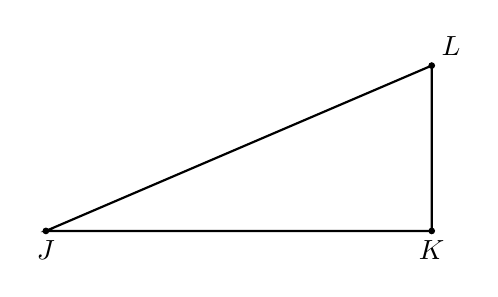
\begin{tikzpicture}[scale=0.7]
            \draw [thick](-1,0)--(6,0)--(6,3)--cycle;
            \draw [fill] (-1,0) circle [radius=0.05] node[below]{$J$};
            \draw [fill] (6,0) circle [radius=0.05] node[below]{$K$};
            \draw [fill] (6,3) circle [radius=0.05] node[above right]{$L$};
          \end{tikzpicture}
        \end{flushright}

  \item Given right $\triangle ABC$ with $m\angle C =90^\circ$, $BC=15$, $m\angle A=41^\circ$. Let $x=AC$. \hfill (2 stars)
    \begin{flushright}
        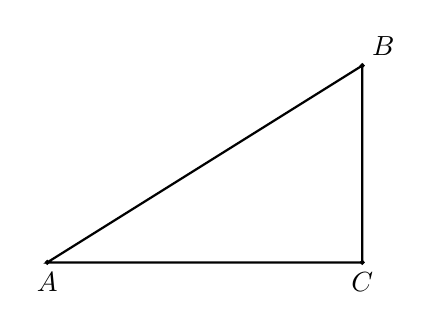
\begin{tikzpicture}[scale=0.5]
          \draw [thick](-1,0)--(7,0)--(7,5)--cycle;
          \draw [fill] (-1,0) circle [radius=0.05] node[below]{$A$};
          \draw [fill] (7,0) circle [radius=0.05] node[below]{$C$};
          \draw [fill] (7,5) circle [radius=0.05] node[above right]{$B$};
        \end{tikzpicture}
      \end{flushright}

  \item Given right $\triangle ABC$ with $m\angle C =90^\circ$, $BC=4$, $AC=19$, and $m\angle A=x^\circ$. \hfill (2 stars)
  \begin{flushright}
    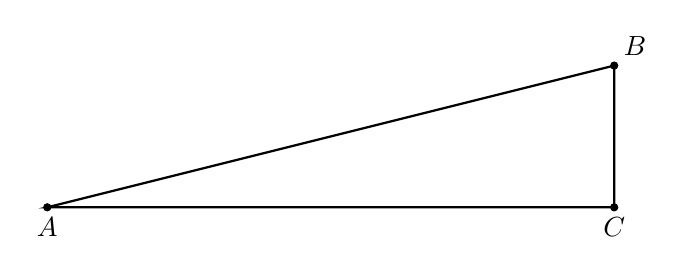
\begin{tikzpicture}[scale=0.9]
      \draw [thick](-1,0)--(7,0)--(7,2)--cycle;
      \draw [fill] (-1,0) circle [radius=0.05] node[below]{$A$};
      \draw [fill] (7,0) circle [radius=0.05] node[below]{$C$};
      \draw [fill] (7,2) circle [radius=0.05] node[above right]{$B$};
    \end{tikzpicture}
  \end{flushright}
  
  \item Given right $\triangle ABC$ with $\overline{AC} \perp \overline{BC}$, $BC=7$, $m\angle B=55^\circ$. Let $x=AC$. \hfill (3 stars)
  \begin{flushright}
    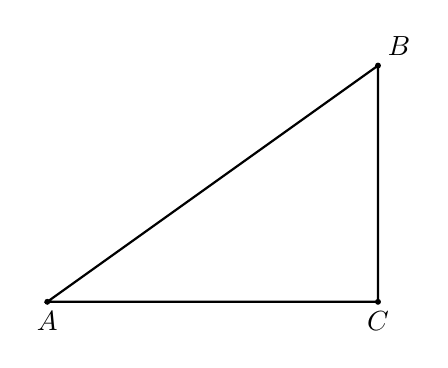
\begin{tikzpicture}[scale=0.6]
      \draw [thick](-1,0)--(6,0)--(6,5)--cycle;
      \draw [fill] (-1,0) circle [radius=0.05] node[below]{$A$};
      \draw [fill] (6,0) circle [radius=0.05] node[below]{$C$};
      \draw [fill] (6,5) circle [radius=0.05] node[above right]{$B$};
    \end{tikzpicture}
  \end{flushright}

\newpage
\subsubsection*{Mixed practice (test tomorrow)}
  \item Convert each equation to slope-intercept form, $y=mx+b$.
    \begin{enumerate}
    \begin{multicols}{2}
      \item $3x+y=2$ (2 stars)\\
      \item $x-4y=12$ (2 stars)
    \end{multicols}     
  \end{enumerate}
    \vspace{3cm}

\item Given $\triangle ABC$ is isosceles but not equilateral with $\angle A \cong \angle C$. \hfill (\emph{not draw to scale})
  \begin{enumerate}
  \item Mark the congruent sides \& angles of $\triangle ABC$. \\[0.25cm]
  Circle True or False:
  \begin{multicols}{2}
  \item True \quad False \quad $\overline{AB} \cong \overline{BC}$
  \item True \quad False \quad $\overline{AB} \cong \overline{AC}$
  \item True \quad False \quad $\overline{BC} \cong \overline{AC}$
  \begin{flushright}
  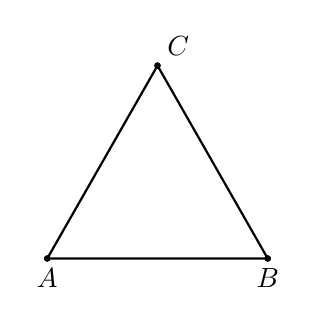
\begin{tikzpicture}[scale=0.7]
    \draw [thick](0,0)--(4,0)--(2,3.5)--(0,0);
    \draw [fill] (0,0) circle [radius=0.05] node[below]{$A$};
    \draw [fill] (4,0) circle [radius=0.05] node[below]{$B$};
    \draw [fill] (2,3.5) circle [radius=0.05] node[above right]{$C$};
  \end{tikzpicture}
  \end{flushright}
  \end{multicols}
  \end{enumerate}

  \item A dilation centered at $A$ maps $\triangle ABC \rightarrow \triangle ADE$. Given the lengths $AC = 6$, $BC = 5$, $AB = 8$, and $CE = 9$. Find $AE$ and then the scale factor $k$. Then find the lengths $AD$ and $DE$. \vspace{1cm}
  \begin{multicols}{2}
    \begin{enumerate}
      \item $AE=$ \vspace{0.3cm}
      \item $k=$ \vspace{0.3cm}
      \item $AD=$ \vspace{0.3cm}
      \item $DE=$ \vspace{0.3cm}

    \end{enumerate}
    \begin{flushright}
      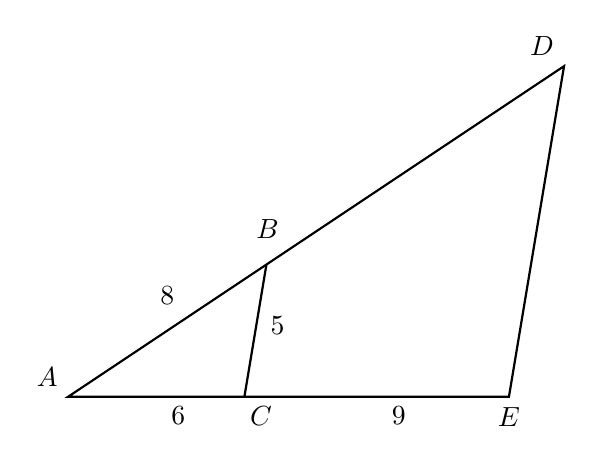
\begin{tikzpicture}[scale=0.7]
        \draw [-, thick] (0,0) node[above left]{$A$}--
        (8,0) node[below]{$E$}--
        (9,6) node[above left]{$D$}--cycle;
        \draw [thick] (3.2,0)--(3.6,2.4);
        \node at (3.5,0) [below]{$C$};
        \node at (4,2.7) [above left]{$B$};
        \node at (2, 0) [below]{$6$};
        \node at (1.8,1.5) [above]{$8$};
        \node at (6, 0) [below]{$9$};
        \node at (3.5, 1.3) [right]{$5$}; \vspace{1cm}
      \end{tikzpicture}
    \end{flushright} 
  \end{multicols}\vspace{1.5cm}

\newpage
  \item \begin{enumerate}
    \item Graph and label the two equations. Mark their intersection as an ordered pair.
      \begin{multicols}{2}
        $y =\frac{2}{3}x-5$ \\
        $y=-2x+3$ \hfill (4 pts)
      \end{multicols}     \vspace{1.5cm}
    \item Find the slopes of the two lines. \hfill (2 points)
      \begin{multicols}{2}
        $m_1=$ \\
        $m_2=$
      \end{multicols}
    \item Are the lines parallel, perpendicular, or neither? Justify your answer with an equation or inequality using the slopes. \hfill (2 points)
    \vspace{1.5cm}
  \end{enumerate}
    \begin{center}
      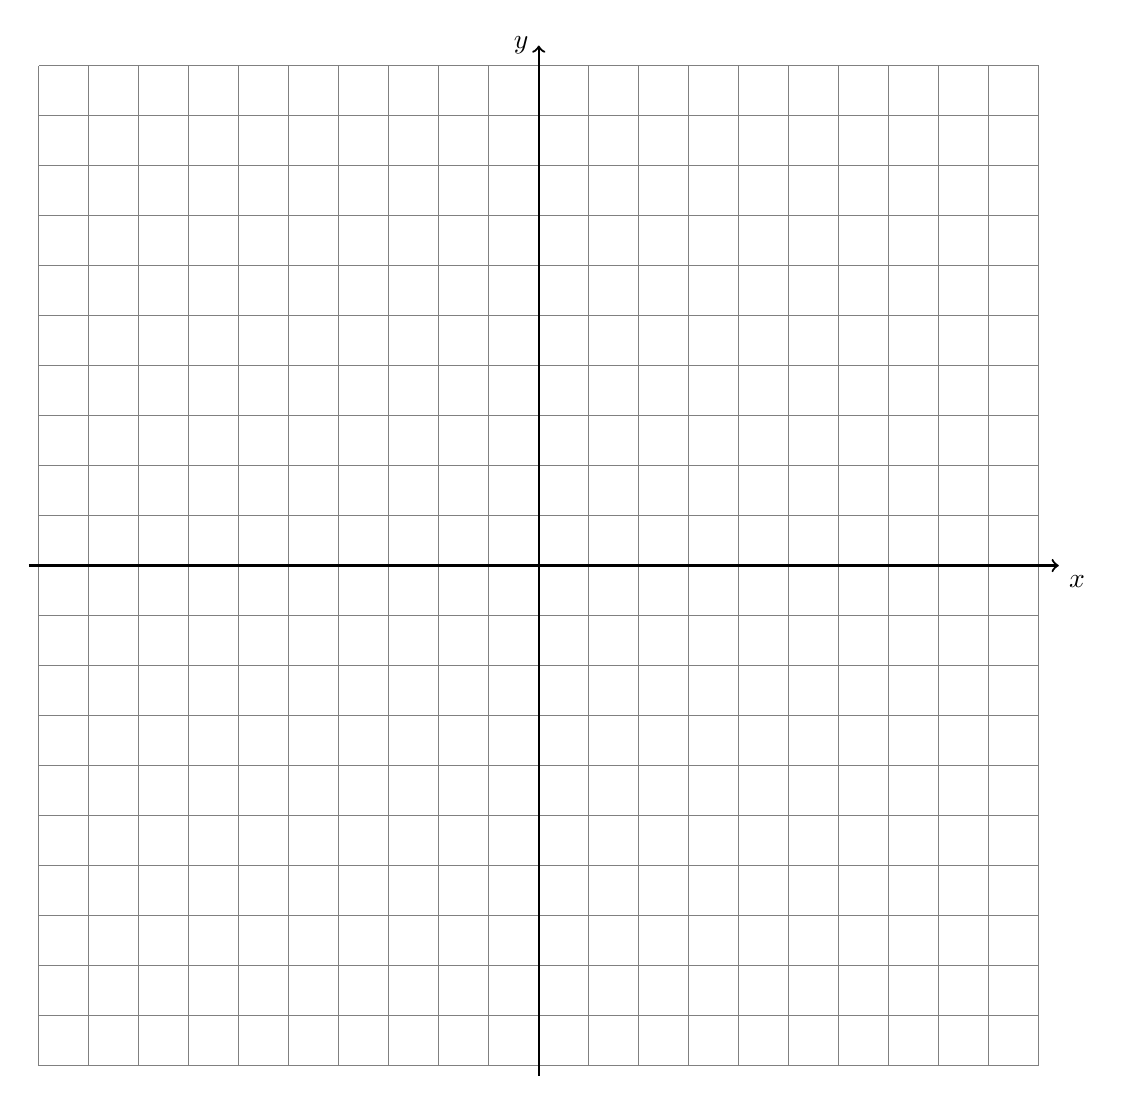
\begin{tikzpicture}[scale=.635]
        \draw [help lines] (-10,-10) grid (10,10);
        \draw [thick, ->] (-10.2,0) -- (10.4,0) node [below right] {$x$};
        \draw [thick, ->] (0,-10.2)--(0,10.4) node [left] {$y$};
      \end{tikzpicture}
    \end{center}
  
\end{enumerate}
\end{document}